Ziel des Versuchs 243 ist es, das thermische Rauschen eines elektrischen Widerstandes auszunutzen, um die Boltzmannkonstante zu bestimmen.

\subsection{Physikalische Grundlagen}

Sobald die Temperatur eines elektrischen Leiters über $0$K ist, führen die Ladungsträger, auch ohne das Anliegen einer äußeren Spannung, zufällige Zick-Zack-Bewegungen aus. Diese Bewegungen führen zu einer Ladungstrennung und somit einer Rauschspannung, welche statistisch um einen Mittelwert $\mean{U_r}$ schwankt. Ohne anliegende Spannung ist die Position der Ladungsträger im Leiter gleichverteilt, es gilt also im zeitlichen Mittel
\begin{align}
  \mean{U_r} = \lim_{t' \to \infty} \frac{1}{t'} \int_0^{t'} U_r(t) \dd{t} = 0.
\end{align}

Der Mittelwert verschwindet somit. Daher wird zur Berechnung der Boltzmannkonstante auf den Effektivwert oder auch Root Mean Square der Rauschspannung
\begin{align}
  \sqrt{\mean{U_r^2}} = \sqrt{\lim_{t' \to \infty} \frac{1}{t'} \int_0^{t'} U_r^2(t) \dd{t}}.
\end{align}
zurückgegriffen. Dieser steht nach der \textit{Nyquist-Beziehung} 
\begin{align}
  \mean{U_r^2} = 4kTR\Delta f
\end{align}
in direkter Relation zur Boltzmannkonstante $k$ und hängt dazu lediglich von der Temperatur $T$, dem Widerstand $R$ des Leiters und der Bandbreite $\Delta f$ der Messelektronik ab.

Da bei der Messung ein Verstärker verwendet wird, welcher selbst wiederum eine Rauschquelle darstellt, setzt sich der gemessene Effektivwert aus dem Rauschen des Widerstands $\mean{U_R^2}$ und des Verstärkers $\mean{U_V^2}$, welcher im Nachhinein abgezogen werden muss, zusammen.

Im späteren Verlauf des Versuchs wird die für $\Delta f$ die Rauschbandbreite $B$ des Messsystems eingesetzt. Die Rauschbandbreite ist definiert durch das Integral 
\begin{align}
  B = \int_0^{\infty} g(f)^2 \dd{f}
\end{align}
über das Quadrat des Frequenzgangs $g(f)$. Dieser ergibt sich wiederum aus dem Verhältnis der Ein- und Ausgangsspannung bei einer bestimmten Frequenz, nach
\begin{align}
  g(f) = \eval{\frac{U_{\text{aus}}}{U_{\text{ein}}}}_f.
\end{align}


\newpage\noindent
\subsection{Versuchsdurchführung}

Die Versuchsdurchführung setzte sich aus drei Teilschritten zusammen. 

\textbf{Versuchtteil 1 / Vorversuch.} Im Vorversuch untersuchten wir zunächst qualitativ die Rauschspannung eines ohm'schen Widerstandes. Hierzu schlossen wir den Widerstand direkt an den Verstärker und den Verstärker ohne einen zusätzlichen Filter an das Oszilloskop an. In der Ausgabe des Oszilloskops war eine gleiche Verteilung aller Frequenzen zu beobachten. Nach Zuschalten des Bandfilters zeichnete sich im Frequenzspektrum ein Abfall bei den höheren Frequenzen ab.

\textbf{Versuchsteil 2.} Im zweiten Versuchsteil ging es um die Bestimmung des Effektivwertes der Rauschspannung. Der zugehörige Versuchsaufbau ist in Abbildung \ref{fig:aufbau_vt2} dargestellt. Für die Widerstandswerte von 5 bis 30 $\si{\kilo\ohm}$ führten wir jeweils eine Messreihe von 110 Punkten durch, um den Mittelwert, sowie die Standardabweichung und den fehler des Mittelwerts zu bestimmen.

\begin{figure}[H]
  \centering
  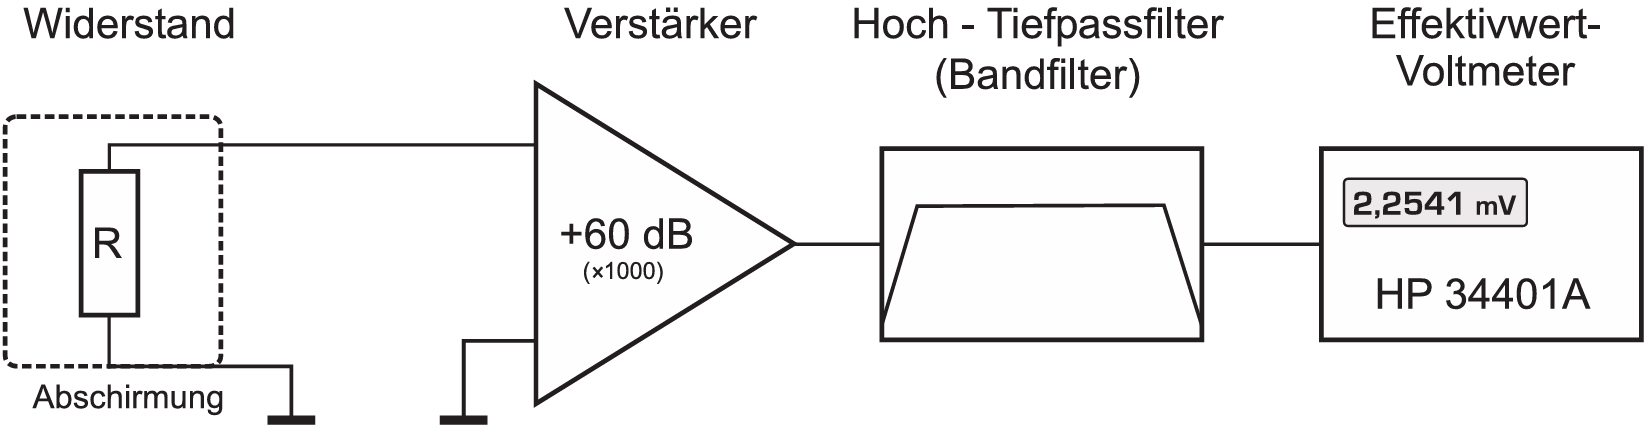
\includegraphics[width=0.8\textwidth]{files/schaltplan_aufgabe2.png}
  \caption{Aufbau Versuchsteil 2}
  \label{fig:aufbau_vt2}
\end{figure}

Die Aufgenommenen Werte sind dem Messprotokoll zu entnehmen.

\textbf{Versuchsteil 3.} Der letzte Versuchsteil umfasste die Bestimmung des Frequenzgangs des Verstärkers und des Bandfilters. Um kontrolle über das Eingangssignal zu haben, verwendeten wir in diesem Versuchsteil einen Funktionsgenerator als Spannungsquelle. Dieser lieferte ein Sinussignal mit einstellbarer Frequenz und Amplitude. Abbilung \ref{fig:aufbau_vt3} zeigt den Aufbau dieses Versuchsteils.

\begin{figure}[H]
  \centering
  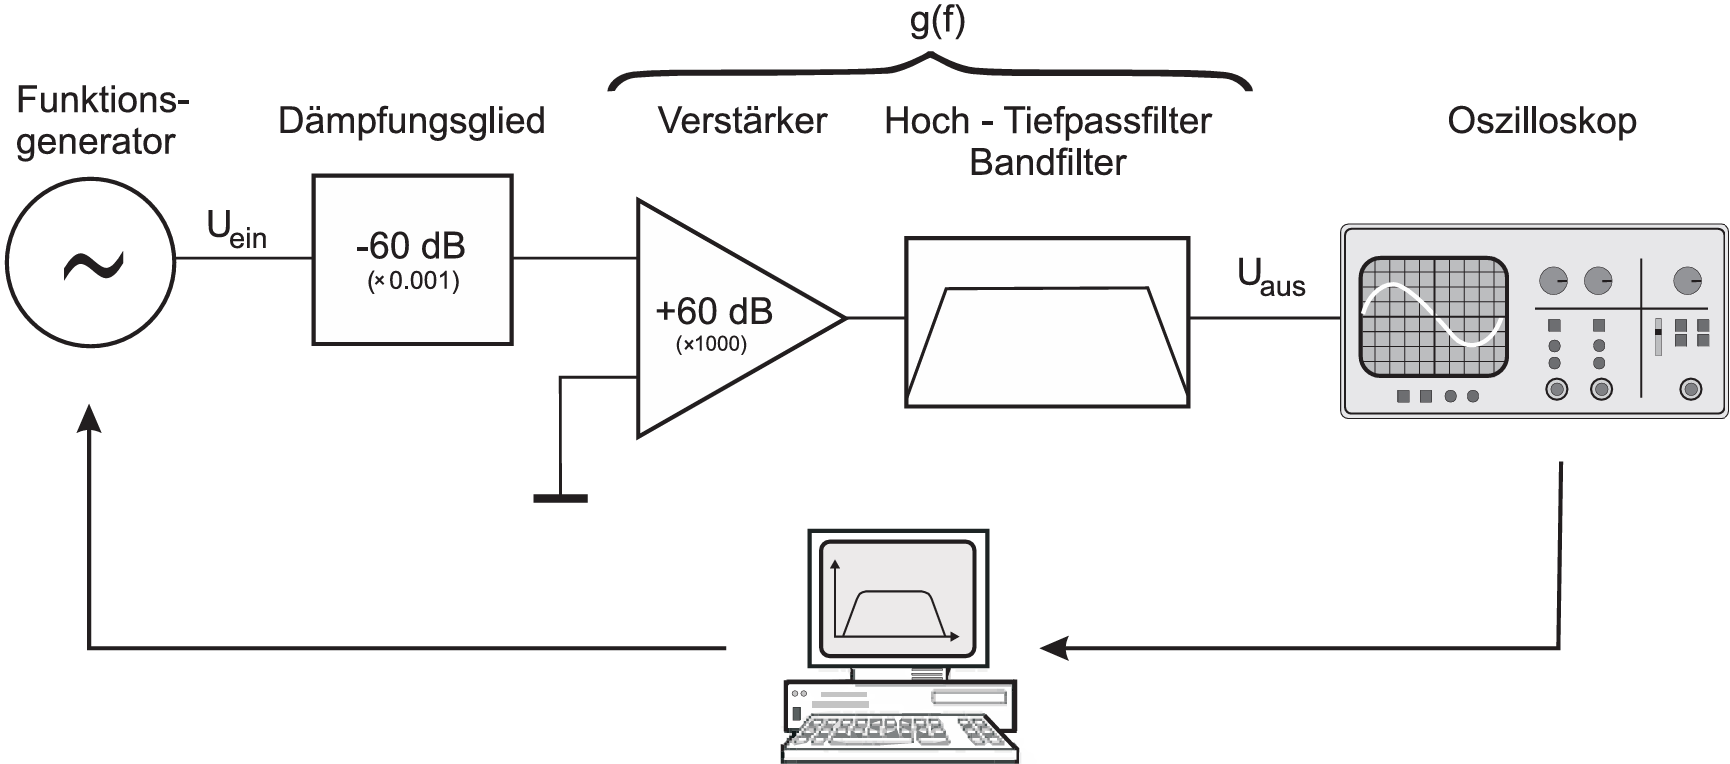
\includegraphics[width=0.8\textwidth]{files/schaltplan_aufgabe3.png}
  \caption{Aufbau Versuchsteil 3}
  \label{fig:aufbau_vt3}
\end{figure}

Die Messungen dieses Versuchsteils wurden durch die Oszilloskopsoftware automatisiert durchgeführt. Diese zeichnete für eine Konstante Eingangsspannung $\sqrt{\mean{U^2_\text{ein}}}$ bei kontinuierlich steigender Frequenz $f$ die Augangsspannung $\sqrt{\mean{U^2_\text{aus}}}$ auf.